\clearpage
\begin{explanationbox}
	\textbf{最低认知负担：把两条焦半径写成「$A+T$、$A-T$」。}

	
\begin{center}
\begin{tikzpicture}[x=1cm,y=1cm,every node/.style={font=\small}]
\path[use as bounding box] (-1.5,-.7) rectangle (10,3.4);
\node[anchor=west] at (-1.3,3) {右支代表：$a_E=4,\ a_H=1$（同尺度长度图）};
\draw[very thick,blue!70!black] (0,2)--(4,2);
\draw[very thick,red!70!black] (4,2)--(5,2);
\draw[very thick,blue!70!black] (0,.6)--(3,.6);
\draw[dashed,red!70!black,thick] (3,.6)--(4,.6);
\foreach \x/\y in {0/2,4/2,5/2,0/.6,3/.6,4/.6} \draw (\x,\y-.12)--(\x,\y+.12);
\node[above] at (2,2) {$a_E$}; \node[above] at (4.5,2) {$a_H$};
\node[below] at (1.5,.6) {$a_E-a_H$}; \node[below] at (3.5,.6) {$a_H$};
\node[anchor=west] at (5.6,2) {$PF_1=a_E+a_H=5$};
\node[anchor=west] at (5.6,.6) {$PF_2=a_E-a_H=3$};
\node[anchor=west] at (-1.3,-.5) {两条长度之和 $=2a_E$；较长边减较短边 $=2a_H$。};
\end{tikzpicture}

\end{center}
把椭圆的半长轴记作 $A=a_E$，双曲线的实半轴记作 $T=a_H$。
\textbf{先问：为什么要求和、求差？}因为两种定义发生在\emph{同一对焦半径}上：
\[
\underbrace{PF_1+PF_2}_{\text{两边总长度}}=2A,\qquad
\underbrace{|PF_1-PF_2|}_{\text{两边长度差}}=2T.
\]
取焦点 $F_1=(-c,0)$、$F_2=(c,0)$，若 $P$ 在\textbf{双曲线右支}，则
$PF_1>PF_2$，于是绝对值可去掉：
\[
\begin{cases}
PF_1+PF_2=2A,\\
PF_1-PF_2=2T.
\end{cases}
\]
\textbf{相加：}消去较短边，$2PF_1=2A+2T$；
\textbf{相减：}消去较长边，$2PF_2=2A-2T$。所以
\[
\boxed{PF_1=A+T},\qquad \boxed{PF_2=A-T}.
\]
\textbf{几何意义：} $A$ 是两条焦半径的\emph{平均长度}，
$T$ 是较长边相对平均值\emph{多出来的长度}（也是较短边少掉的长度）。
左支只交换“长、短边”的身份，余弦定理用的是两边平方和及其乘积，结果不变。

	\textbf{为什么现在用余弦定理？}已掌握焦点三角形\emph{两腰} $A\pm T$、
它们的\emph{夹角} $\theta$，而要联系\emph{对边} $F_1F_2=2c$，正适用
“两边及夹角求对边”的余弦定理：
\[
(2c)^2=(A+T)^2+(A-T)^2-2(A+T)(A-T)\cos\theta.
\]
平方和与乘积分别是
\[
(A+T)^2+(A-T)^2=2(A^2+T^2),\quad
(A+T)(A-T)=A^2-T^2.
\]
所以重新按 $A^2,T^2$ 分组，得到
\[
2c^2=A^2(1-\cos\theta)+T^2(1+\cos\theta).
\]
\textbf{角度为什么与和差配对？}总长度对应 $A^2(1-\cos\theta)$，
长度差对应 $T^2(1+\cos\theta)$，来自上述平方和、平方差的分组，
不是需要死记的符号口诀。最后代入 $A=c/e_1,T=c/e_2$ 即消去共同尺度 $c$。

	\textbf{本质：}椭圆控制\textbf{和}，双曲线控制\textbf{差}，
	两者在同一个焦点三角形上同时成立，就可以把未知焦半径完全消掉。
\end{explanationbox}

\clearpage
\begin{explanationbox}
	\textbf{精确坐标图（$F_1=(-2,0),F_2=(2,0),P=(2,3)$）。}
	\begin{center}
		% 精确坐标：共焦点 F1=(-2,0), F2=(2,0)
% 椭圆 E: x^2/16 + y^2/12 = 1 (e1=1/2)
% 双曲线 H: x^2 - y^2/3 = 1 (e2=2)
% P=(2,3), PF1=5, PF2=3, F1F2=4, cos(theta)=3/5
% 所有几何点与图形由真实方程指定，并非自由手绘。
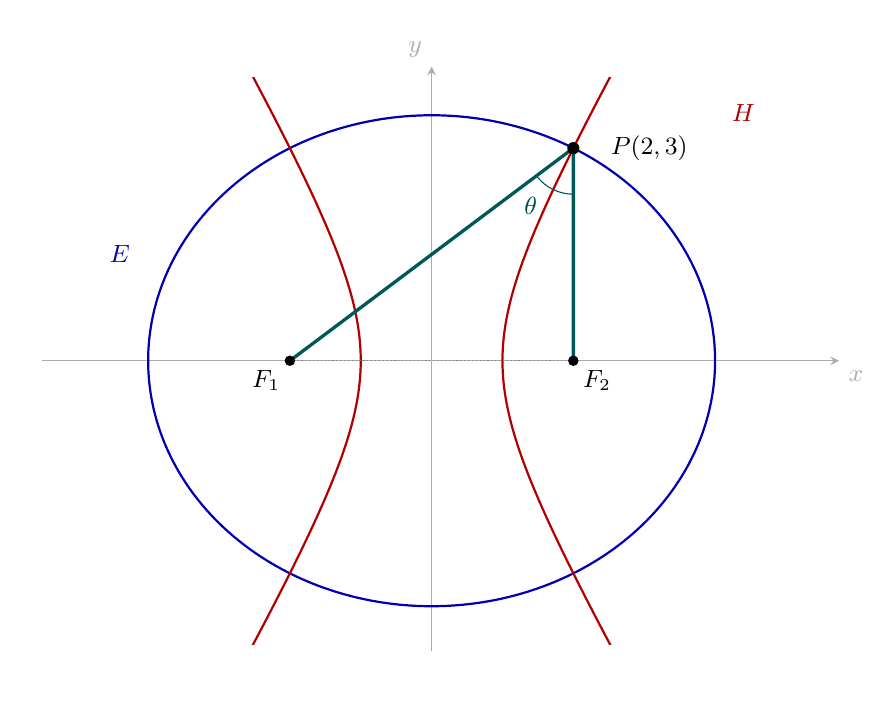
\begin{tikzpicture}[x=0.9cm,y=0.9cm,>=stealth,every node/.style={font=\small}]
  \path[use as bounding box] (-5.7,-4.5) rectangle (6.0,4.7);
  \draw[->,gray!65,thin] (-5.5,0)--(5.75,0) node[below right] {$x$};
  \draw[->,gray!65,thin] (0,-4.1)--(0,4.15) node[above left] {$y$};
  \begin{scope}
  \clip (-5.2,-4) rectangle (5.2,4);
  \draw[thick,blue!70!black,domain=0:360,samples=181,smooth,variable=\t]
    plot ({4*cos(\t)},{sqrt(12)*sin(\t)});
  \draw[thick,red!70!black,domain=-70:70,samples=131,smooth,variable=\t]
    plot ({1/cos(\t)},{sqrt(3)*tan(\t)});
  \draw[thick,red!70!black,domain=-70:70,samples=131,smooth,variable=\t]
    plot ({-1/cos(\t)},{sqrt(3)*tan(\t)});
  \end{scope}
  \coordinate (Fone) at (-2,0);
  \coordinate (Ftwo) at (2,0);
  \coordinate (PP) at (2,3);
  \draw[very thick,teal!70!black] (PP)--(Fone) (PP)--(Ftwo);
  \draw[thin,densely dotted,gray] (Fone)--(Ftwo);
  \fill[black] (Fone) circle(1.9pt) node[below left] {$F_1$};
  \fill[black] (Ftwo) circle(1.9pt) node[below right] {$F_2$};
  \fill[black] (PP) circle(2.2pt) node[right,xshift=10pt] {$P(2,3)$};
  \draw[teal!70!black] (2,2.35) arc[start angle=-90,end angle=-143.130102,radius=0.65];
  \node[teal!60!black] at (1.40,2.18) {$\theta$};
  \node[blue!70!black] at (-4.4,1.5) {$E$};
  \node[red!70!black] at (4.4,3.5) {$H$};
\end{tikzpicture}

	\end{center}
	\[
		E:\ \frac{x^2}{16}+\frac{y^2}{12}=1,\qquad
		H:\ x^2-\frac{y^2}{3}=1.
	\]
	这两条曲线共享 $c=2$，交点 $P=(2,3)$ 处有
	\[
		PF_1=5,\ PF_2=3,\ F_1F_2=4,\quad e_1=\frac12,\ e_2=2.
	\]
	由余弦定理 $\cos\theta=3/5$、$\sin\theta=4/5$。
	于是 $1/e_1+1/e_2=5/2=2/\sin\theta$：\textbf{此图恰好演示等号成立}。

	\textbf{为何此图取到等号？} $e_1e_2=(1/2)\cdot2=1$；
并且 $P=(2,3)$ 与 $F_2=(2,0)$ 在同一竖直线上，
$PF_2\perp F_1F_2$，所以\emph{焦点 $F_2$ 处为直角}。
要区分：$\theta$ 位于 $P$，所以 $\theta$ 仍为锐角，
并不是 $\angle PF_2F_1$。

\textbf{图形辨别：}图中 $\theta$ 是点 $P$ 处\emph{两条焦点连线}的夹角，
\textbf{不是椭圆切线与双曲线切线的夹角}（后者在交点处正交）。
\end{explanationbox}

\clearpage
\begin{explanationbox}
	\textbf{由主公式看可行范围。}
	
\begin{center}
\begin{tikzpicture}[every node/.style={font=\small}]
\begin{axis}[width=11cm,height=6cm,xmin=.44,xmax=1.08,ymin=.7,ymax=5,
 axis lines=left,xlabel={$e_1$},ylabel={$e_2$},xtick={.5,1},ytick={1,2,3,4},clip=false]
\addplot[blue!70!black,very thick,domain=.508:1,samples=160] {sqrt(3)/2/sqrt(1-1/(4*x*x))};
\addplot[red!70!black,dashed] coordinates {(.5,.7)(.5,5)};
\addplot[gray,dashed] coordinates {(.5,1)(1.05,1)};
\addplot[only marks,mark=o,mark size=3pt,thick] coordinates {(1,1)};
\node[anchor=west] at (axis cs:.66,3.8) {$\theta=60^\circ$（固定）};
\node[anchor=west] at (axis cs:.66,3.1) {$\frac12<e_1<1,\quad e_2>1$};
\node[anchor=west] at (axis cs:.53,4.65) {$e_1\to\frac12^+:\ e_2\to+\infty$};
\node[anchor=west] at (axis cs:.73,1.7) {空心点 $(1,1)$ 不取};
\end{axis}
\end{tikzpicture}

\end{center}
设 $\alpha=\theta/2$，$s=\sin\alpha$，$t=\cos\alpha$，则
	\[
		\frac{s^2}{e_1^2}+\frac{t^2}{e_2^2}=1.
	\]
	若已知 $\theta$ 与 $e_1$，可直接解出
	\[
		\boxed{e_2=\frac{\cos(\theta/2)}{
				\sqrt{1-\sin^2(\theta/2)/e_1^2}}}.
	\]
	因为 $e_2>1$、$e_1<1$，固定 $0<\theta<\pi$ 后
	\[
		\boxed{\sin\frac\theta2<e_1<1},\qquad e_2>1.
	\]
\textbf{为什么两个端点不能取？}
\begin{itemize}
\item $e_1=\sin(\theta/2)$ 时第一项等于 $1$，第二项必须为 $0$；
但 $\cos(\theta/2)>0$，只有 $e_2\to+\infty$ 才能逼近，
即双曲线实半轴 $T=c/e_2\to0$，非退化双曲线不能取到。
\item $e_1\to1^-$ 时由主式有 $e_2\to1^+$；
此时椭圆半短轴、双曲线虚半轴分别趋于零：
\[
\sqrt{A^2-c^2}\to0,\qquad \sqrt{c^2-T^2}\to0.
\]
两种非退化曲线都逼近退化边界。
\end{itemize}
\textbf{理解重点：}公式可以\emph{趋近}某个边界，不等于实际存在一条
满足题设的非退化曲线可以\emph{取到}该边界。
\end{explanationbox}

\clearpage
\begin{explanationbox}
\textbf{从余弦式到加权平均：为什么半角形式更有几何感？}

令 $A=a_E,T=a_H$，余弦定理化简为
\[
2c^2=A^2(1-\cos\theta)+T^2(1+\cos\theta).
\]
把 $1\mp\cos\theta$ 换成半角平方：
\[
\boxed{c^2=A^2\sin^2\frac\theta2+T^2\cos^2\frac\theta2}.
\]
由于 $\sin^2(\theta/2)+\cos^2(\theta/2)=1$ 且两个权重均严格为正，
这是 $A^2$ 和 $T^2$ 的\textbf{加权平均}。
因此 $T^2<c^2<A^2$，即 $T<c<A$。

同一个大小关系还可以直接由\emph{三角形不等式}读出：
\[
|PF_1-PF_2|<F_1F_2<PF_1+PF_2
\quad\Longrightarrow\quad 2T<2c<2A.
\]
\textbf{两种视角对应同一几何事实：}在非退化焦点三角形中，
底边 $2c$ 必须严格夹在“两腰之差”和“两腰之和”之间。
所以离心率自然满足 $e_1=c/A<1$ 与 $e_2=c/T>1$。

\textbf{教师拓展（为何两曲线在交点处正交）：}
令 $\mathbf u_1,\mathbf u_2$ 为从焦点 $F_1,F_2$ 指向 $P$ 的
两个单位向量。椭圆是 $PF_1+PF_2$ 的等值线，故其法线沿
$\mathbf u_1+\mathbf u_2$；双曲线是 $PF_1-PF_2$ 的等值线，
故其法线沿 $\mathbf u_1-\mathbf u_2$（左支方向取负也不影响）。
而
\[
(\mathbf u_1+\mathbf u_2)\cdot(\mathbf u_1-\mathbf u_2)
=|\mathbf u_1|^2-|\mathbf u_2|^2=1-1=0.
\]
所以两条曲线的法线互相垂直，切线也互相垂直。
\textbf{注意：}此正交是\emph{曲线切线}的夹角，不是焦角 $\theta$。
\end{explanationbox}
